
\فصل{روش پیشنهادی}

‌
‌
همیشه یکی از چالش‌های مهم در پیاده‌سازی مدل‌های مختلف به خصوص روی 
\trans{کلان‌داده}{Bigdata}
انتخاب مدلی با کمترین پیچیدگی است. به همین دلیل در طراحی سیستم جدید، به سراغ مدل‌های سنگین‌تر مانند
BERT
نرفتیم  و تلاش کردیم تا همان مدل قبلی بر پایه LSTM‌ را بهبود داده و قابلیت‌های جدیدی مثل فرایند تایید خودکار را به آن اضافه کنیم تا به یک مدل به اصطلاح بی‌درنگ برسیم.

اما اضافه کردن فرایند تایید خودکار نظرات کار ساده‌ای نیست. چون می‌تواند هزینه‌های مستقیم و غیرمستقیم زیادی را به شرکت تحمیل کند. پس باید یک 
\trans{پس‌پردازش}{Post-Processing}
هم برای کاهش خطاهای احتمالی در نظر می‌گرفتیم که در ادامه، بیشتر از آن صحبت می‌کنیم.

حال در این قسمت نیاز است تا نگاهی دقیق به ساختار کلی مدل بیاندازیم:

\section{مرحله اول: انتخاب ویژگی}

\trans{انتخاب ویژگی}{Feature Selection} 
همان فرایند انتخاب زیرمجموعه‌ای از ویژگی‌های مرتبط برای ساخت مدل است. ما در این فرایند، چند ویژگی مشخص را به عنوان ورودی مدل انتخاب کردیم که عبارت‌اند از:

\begin{itemize}
    \item محتوای نظر
    \item نقاط ضعف و قوت نظر
    \item عنوان نظر
    \item گروه کالایی کالا
    \item عنوان کالا
    \item خریدار بودن یا نبودن شخصی که نظر را ثبت کرده

\end{itemize}

در نهایت خروجی، میزان احتمال تایید شدن نظر ورودی را تخمین می‌زند.

\begin{figure}[H]
\centering
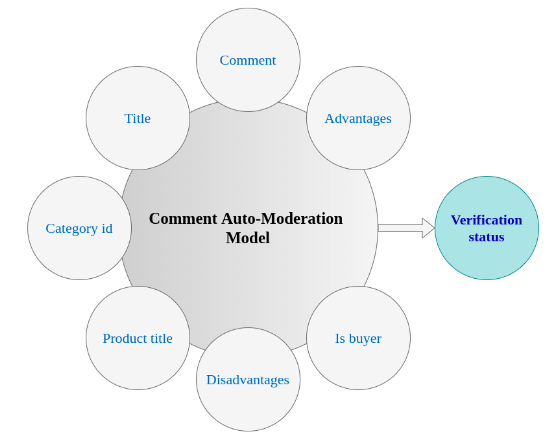
\includegraphics[width=15cm]{figs/auto_moderation_model.png}
\caption{مدل تایید خودکار}\label{}
\label{fig:test}
\end{figure}

با پشت سر گذاشتن مرحله اول یعنی انتخاب ویژگی، به مرحله دوم می‌رسیم. مرحله‌ای که باید از پیش‌پردازش بیش‌تر بگوییم..

\section{مرحله دوم: پیش پردازش}

در مدل‌های متنی معمولا یک مرحله پیش‌پردازش وجود دارد. پیش‌پردازشی که ما روی متن‌های نظرات انجام می‌دهیم از دو بخش تشکیل شده‌ است.
در بخش اول که به اصطلاح به آن \لر {Normalizer} گفته می‌شود، سعی می‌کنیم از پیچیدگی‌های اضافی ورودی کم کنیم. برای مثال اعداد انگلیسی به فارسی تبدیل می‌شود، علائم نگارشی از کلمات جدا می‌شود، «ی» عربی به فارسی تبدیل می‌شود و… .
اما بخش دوم یا \لر{Tokenizer}، کمی مفصل‌تر است. در نظر بگیرید که هر ویژگی متنی توزیع جداگانه‌ای دارد و یکی از ویژگی‌های ما مثل «گروه کالایی محصول» هم متنی نیست. برای این مسئله به طور خلاصه، هر کدام از ویژگی‌های متنی به یک \لر{Tokenizer} و سپس \لر{Indexer} وصل می‌شود که در فرایند \لر{Tokenizing}، بخش \لر{Indexing} درست می‌شود که این بخش هم به \لر{Embedding} مدل وصل می‌شود.
اما سوالی که به وجود می‌آید، این است که ویژگی عنوان کالایی محصول یا همان \لر{Category ID } را چگونه به مدل دهیم؟ همان‌طور که می‌دانید اولین راه‌حل برای ویژگی‌های چند مقداری یا \لر{Categorical}، استفاده از الگوریتم
 \لر{One-Hot Encoder}
  است؛ اما در دیجی‌کالا تعداد همه‌ی عنوان‌های کالا بسیار زیاد است و این کار خیلی منطقی نیست. 
راه‌حلی که ما استفاده کردیم این بود که به ویژگی «عنوان کالا» به عنوان یک متن نگاه کرده و به یک بردار ۶۴تایی 
\trans{نگاشت}{mapping}
 می‌کنیم؛ این بردار در طول فرایند یادگیری آموزش می‌بیند.

\section{مرحله سوم: معماری مدل}
ساختار مدل پیشنهادی را می‌توانید در شکل زیر ببینید:

\begin{figure}[H]
\centering
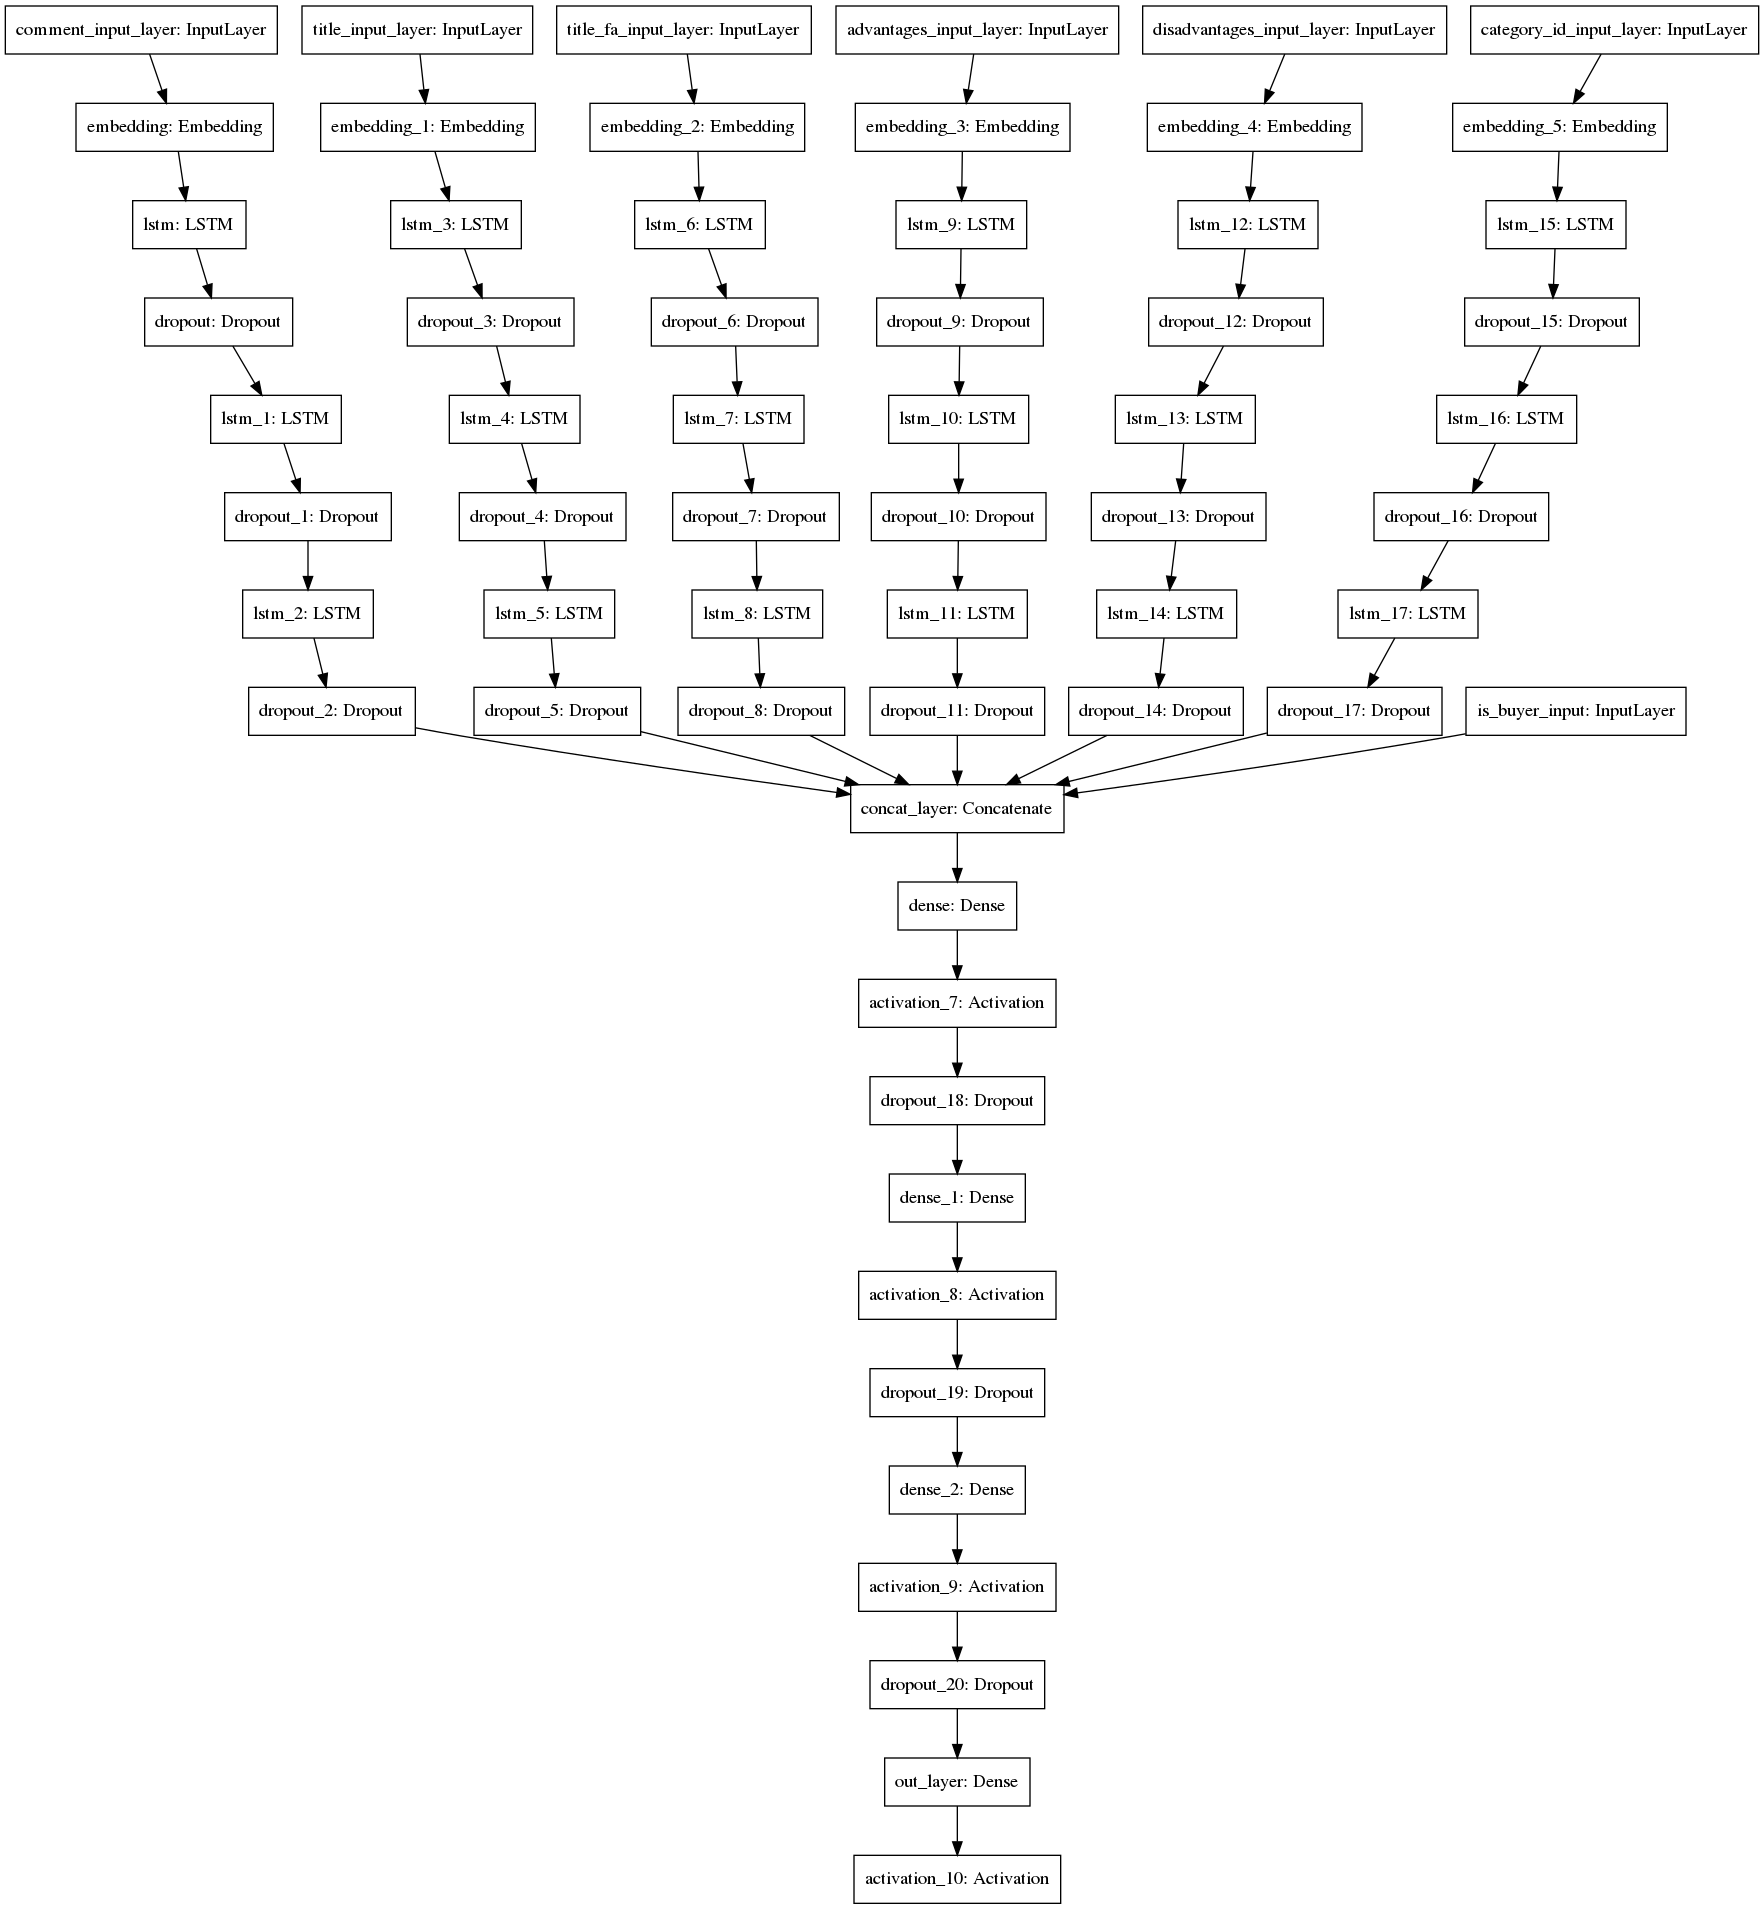
\includegraphics[width=15cm]{figs/Model1.png}
\caption{معماری مدل پیشنهادی}\label{}
\label{fig:test}
\end{figure}

همان‌طور که در بلوک دیاگرام مدل قابل مشاهده است، هرکدام از بخش‌های مبتنی بر متن ورودی، پس از گذر از لایه \لر{Embedding}، وارد یک زیر شبکه‌ی شامل سه لایه \لر{LSTM} می‌شود. پس خروجی هر زیر شبکه \لر{LSTM} در کنار هم قرار می‌گیرند و آخرین ورودی که خریدار بودن یا نبودن کاربر را تعیین می‌کند و تک نورون است هم در کنار سایر خروجی‌های مختلف قرار می‌گیرد.

خروجی شبکه مقدار احتمال تایید شدن نظر ورودی است. برای تعیین وضعیت نظرات از روی خروجی شبکه، دو مقدار \لر{Threshold} برای تایید و رد، در نظر گرفته شده‌ است که نظراتی که احتمال تایید آن‌ها بین این دو مقدار قرار می‌گیرد، به معنای عدم اطمینان مدل در تصمیم‌گیری هستند و برای بررسی بیشتر برای کارشناس‌ها ارسال می‌شوند.


\section{مرحله چهارم: پس پردازش}
در مرحله پس‌پردازش به دنبال کاهش مثبت‌های کاذب یا 
\لر{False Positive}
هستیم. در واقع در این مرحله، می‌خواهیم نظرات نامناسبی که به هیچ وجه نباید تایید شوند را مشخص کنیم. برای این کار از \لر{Tokenizer} یک مدل \لر{BERT} استفاده کردیم تا ریشه عبارت‌های نامناسب را پیدا کنیم. سپس این نظرات در چند فهرست قرار می‌گیرند که این فهرست‌ها شامل کلمات نامناسب و سایر عبارت‌های غیرقابل انتشار هستند. سپس این کلمات بررسی شده و اگر تایید شوند، مدل تایید نهایی را ارایه می‌دهد.
برای مثال در کلمه‌ «نشستندی»، توکنایزر این کلمه را  به صورت «نشست + ندی» تقسیم می‌کند و اگر کلمه «نشست» در فهرست سیاه باشد،  تمام مشتقات این کلمه را تا حد خوبی شناسایی کرده و نظراتی که دارای این مشتقات هستند را مستقیما برای کارشناس ارسال می‌کند.

\section{مرحله پنجم: شناسایی تولیدکنندگان نظرات نامناسب}
یکی از مشکلاتی که ما در بخش نظرات با آن روبه‌رو هستیم، این است که بعضی کاربران به دلایل مختلف مثل دریافت امتیاز دیجی‌کلاب، تخریب کالای رقیب و... به تولید تعداد زیادی نظر می‌پردازند. برای حل این مشکل معیاری به عنوان \لر{Spammer} بودن تعریف می‌کنیم.
معیاری که توسط آن، احتمال \لر{Spammer} بودن هر کاربر مشخص می‌شود، به صورت زیر تعریف شده است:

\begin{equation}
user \: performance = \dfrac{number \: of \: verified \: comments}{total \: number \: of \: submitted \: comments}
\end{equation}

پس مقدار بازدهی هر کاربر در بازه زمانی مشخصی محاسبه شده و باتوجه‌به نمودار زیر، وضعیت  \لر{Spammer} بودن آن تعیین می‌شود.


\begin{figure}[H]
\centering
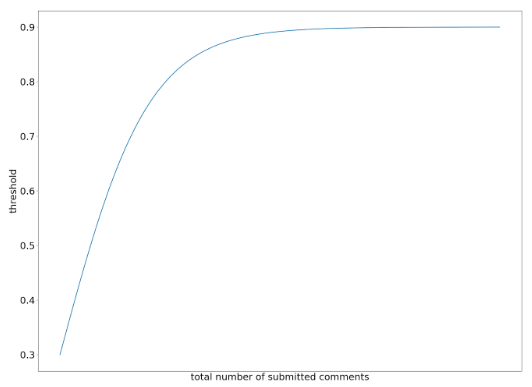
\includegraphics[width=15cm]{figs/spammer.png}
\caption{نمودار نسبت تعداد کل نظرات به نظرات تایید شده}\label{}
\label{fig:test}
\end{figure}

نمودار بالا مقدار \لر{Threshold} برای تصمیم‌گیری در مورد \لر{Spammer} بودن هر کاربر را تعیین می‌کند. مقدار این \لر{Threshold} به صورت داینامیک و باتوجه‌به تعداد کل نظرات ثبت شده توسط هر کاربر در بازه زمانی مورد نظر به دست می‌آید. 
طبق نمودار، هرچه تعداد کل نظرات ثبت شده توسط کاربر بیشتر باشد، بازدهی مورد انتظار از آن کاربر هم بیشتر می‌شود. در نهایت اگر مقدار بازدهی کاربر مورد نظر کمتر از \لر{Threshold} آن کاربر باشد، به عنوان \لر{Spammer} شناسایی شده و برای کارشناس به منظور بررسی دقیق‌تر فرستاده می‌شود. 
غیر خطی بودن این نمودار به این دلیل است که با تعداد نظرات کم، \لر{Threshold} بالاتری در نظر گرفته‌ شود و شناسایی کمتری انجام شود.


\section{مرحله ششم: مدل BERT خلاقانه}

برای 
\trans{بررسی احساسات و معنا}{Intent sentiment analysis}
ی نظرات از یک سری شاخص استفاده می‌کنیم:

\begin{figure}[H]
\centering
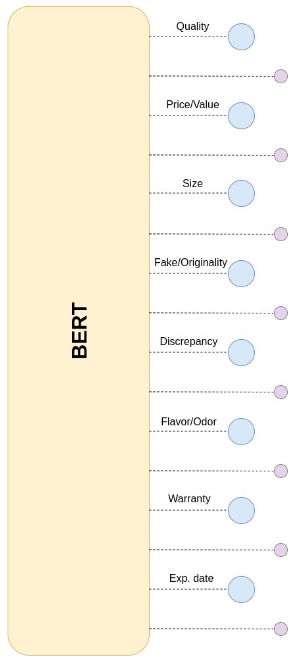
\includegraphics[width=10cm]{figs/bert_model.png}
\caption{مدل پیشنهادی \لر{BERT}در حالت جدید}\label{}
\label{fig:test}
\end{figure}

این \لر{intent}ها عبارتند از:
\begin{enumerate}
    \item کیفیت
    \item ارزش خرید نسبت به قیمت
    \item ابعاد
    \item اصالت کالا
    \item مغایرت کالا با کالای خریداری شده
    \item طعم/بو
    \item گارانتی
    \item تاریخ انقضا
\end{enumerate}


در حالت کلی برای هر یک از 
\لر{intent}ها 
سه
\لر{sentiment}
داریم که عبارتند از حالت‌های مثبت، منفی و خنثی. با توجه به ۸
\لر{intent}ای که در بالا بدان اشاره شد، اگر بخواهیم هر کدام را به‌صورت مجزا در نظر بگیریم، ۲۴ خروجی خواهیم داشت (زیرا ۸ شاخص داریم که هر کدام ۳ حالت مثبت، منفی و یا خنثی را می‌توانند داشته باشند) که اولا خروجی مدل شبکه را بسیار سنگین و 
 \trans{پراکنده}{sparse}
می‌کند و ثانیا شبکه به درستی آموزش داده نمی‌شود. از همین رو، روش خلاقانه‌ای که در این مدل از آن استفاده کردیم، پیش‌بینی 
\لر{intent}ها از روی متن و پس از آن تشخیص احساسات از روی آن شاخص بود. 
 به بیان دیگر، اول بررسی می‌شود که کدام شاخص‌ها در متن به کار رفته‌اند؛ برای مثال، ابتدا در نظر بررسی می‌شود که آیا کلمه‌ای به کار رفته است که به مفهوم کیفی یک کالا اشاره کند یا خیر و سپس در صورتی که جواب مثبت باشد، بررسی می‌شود که آیا آن کلمه مثبت، منفی و یا خنثی بوده است. استفاده از این روش ساده و خلاقانه، باعث بهبود خروجی شبکه که باعث افزایش سرعت و دقت مدل نهایی می‌شود.

با توجه به مطالبی که در بند قبل به آن اشاره کردیم، پروژه‌ی حال حاضر 
یادگیری ماشین \trans{چند وظیفه‌ای}{multi task}
است؛ زیرا دو تا کار تحلیل احساسات و تشخیص شاخص‌ها به‌صورت هم‌زمان در حال اجرا هستند. یادگیری چندوظیفه‌ای زیر مجموعه‌ای از یادگیری ماشین است که در آن چندین کار یادگیری همزمان حل می‌شود، در حالی که از نقاط اشتراک و تفاوت بین وظایف استفاده می‌شود. این می‌تواند باعث بهبود کارایی یادگیری و دقت پیش‌بینی برای مدل‌های خاص وظیفه شود، در مقایسه با آموزش مدل‌ها به‌طور جداگانه. نسخه‌های اولیه یادگیری چندوظیفه‌ای «اشاره» نامیده می‌شدند.
\cite{wiki1}
\cite{wiki2}
\cite{wiki3}
به کارگیری تحلیل احساسات و تشخیص شاخص‌ها در کنار یک‌دیگر به ما این امکان را می‌دهد تا این شبکه‌ها به یک‌دیگر کمک کنند تا یادگیری بهتری در کل داشته باشیم.

برای اندازه‌گیری دقت مدل باید از یک 
\trans{تابع هزینه}{loss function}
استفاده کنیم. تابع هزینه‌ای که برای مدل در نظر گرفته‌ایم به شکل زیر است:

\begin{equation}
loss = intent \: loss + optimized \: sentiment \: loss
\end{equation}

\begin{equation}
optimized \: sentiment \:loss = intent \: label \times sentiment \: loss
\end{equation}

در فصل بعدی به بررسی نتایج به دست‌آمده با استفاده از این روش خواهیم پرداخت.